\documentclass[10pt,a4paper]{article}
\usepackage[utf8]{inputenc} % para poder usar tildes en archivos UTF-8
\usepackage[spanish]{babel} % para que comandos como \today den el resultado en castellano
\usepackage[margin=2cm]{geometry}
\usepackage{amsmath}
\usepackage{listings}
\usepackage{color}
\usepackage{graphicx}
\usepackage{wrapfig}
\usepackage{algorithm}
\usepackage{algpseudocode}
\usepackage{mathtools}

\begin{document}

\definecolor{dkgreen}{rgb}{0,0.6,0}
\definecolor{gray}{rgb}{0.5,0.5,0.5}
\definecolor{mauve}{rgb}{0.58,0,0.82}
\lstset{frame=tb,
  language=Java,
  aboveskip=3mm,
  belowskip=3mm,
  showstringspaces=false,
  columns=flexible,
  basicstyle={\small\ttfamily},
  numbers=none,
  numberstyle=\tiny\color{gray},
  keywordstyle=\color{blue},
  commentstyle=\color{dkgreen},
  stringstyle=\color{mauve},
  breaklines=true,
  breakatwhitespace=true,
  tabsize=3
}

\section{Genkidama}

\subsection{Descripción del problema}

El problema a resolver es el siguiente:
Tenemos un secuencia de puntos $(x,y)$ en el espacio para los cuales, si la coordenada $x$ de un punto es mayor a la de otro punto, la coordenada en y del segundo punto es menor. Dado un valor $T$, se desea calcular la minima cantidad de genkidamas a tirar para destruir a todos los puntos. Si se tira a un punto $(x_{0},y_{0})$ la genkidama alcanza a destruir a todos los puntos que posean $x \leq x_{0} + T$ y posean $y \leq y_{0} + T$.\\

\subsection{Ejemplos}

Supongamos que tenemos los puntos mostrados en la Figura 1 y $T = 1$.\\
\begin{figure}[h!]
  \centering
  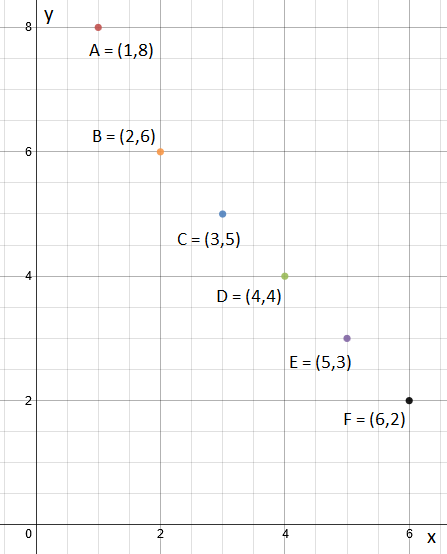
\includegraphics[width=7cm, height=6cm]{EjemploInicialUtil}
  \caption{Puntos distribuidos inicialmente.}
\end{figure}

Primero queremos destruir al objetivo situado en $A$. Miramos el objetivo $B$, que tiene la mayor coordenada $y$ de los que tienen menor coordenada $y$ que $A$ (que son todos dado que se empieza queriendo destruir al objetivo situado en el punto con mayor $y$). En la Figura 2 vemos que $A_{y} > B_{y} + T$ y que A no pertenece al área de impacto A(B, 1), o sea que disparar una genkidama al punto B no eliminaría al androide de A. Por transitividad, como $B_{y} > C_{y} > ... > F_{y}$, ninguno de los disparos a los puntos siguientes a B eliminará al objetivo de A, por lo que es necesario disparar una genkidama a A. El área de impacto A(A, T) = A( (1,8), 1) de esta genkidama, sombrada con rojo en la Figura 2, incluye al punto B, que además es el de mayor coordenada $x$ de los destruidos por esta gendikama.\\
\par{El siguiente a B, C, es el de mayor coordenada $y$ de los que están vivos, y se repite el proceso que se llevó a cabo con A. En la Figura 3 se ve que la segunda gendikama se disparará a D, destruyendo a los objetivos de C, D y E.
Finalmente queda la situación mostrada en la Figura 4 y se dispara una tercera genkidama a F.}\\

\begin{figure}[h!]
\centering
\begin{minipage}{.5\textwidth}
  \centering
  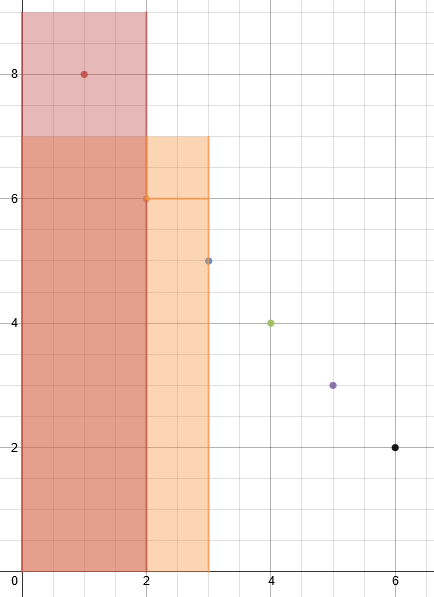
\includegraphics[width=.4\linewidth]{EjemploArea1}
  \caption{Área de impacto de A en rojo y de B en naranja.}
  \label{fig:test1}
\end{minipage}%
\begin{minipage}{.5\textwidth}
  \centering
  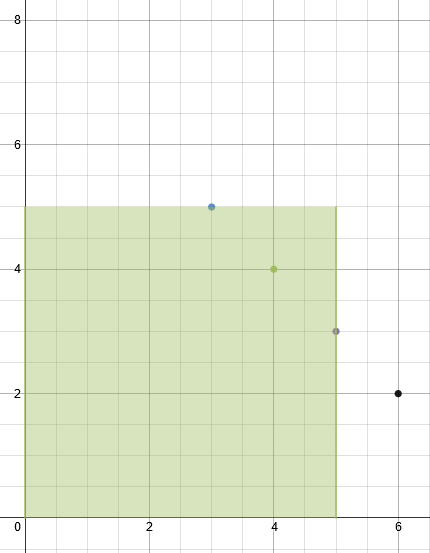
\includegraphics[width=4cm]{EjemploArea2}
  \caption{Área de impacto de D en verde.}
  \label{fig:test2}
\end{minipage}

\end{figure}

\begin{figure}[h!]
\centering
\begin{minipage}{.5\textwidth}
  \centering
  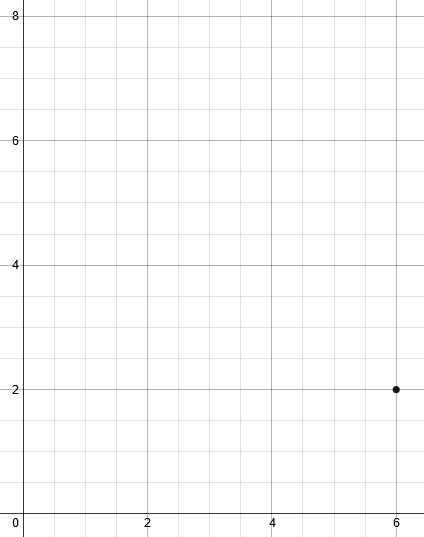
\includegraphics[width=4cm]{EjemploArea3}
  \caption{Androide restante por destruir, en F.}
  \label{fig:test2}
\end{minipage}
\end{figure}

Ahora veamos cómo sería este proceso con $T = 2$.
De vuelta se comienza queriendo destruir al objetivo en A. Como se ve en la Figura 5, disparar a C no destruye a A pero disparar a B sí. Así, morirán los androides situados en los puntos incluidos en la región sombreada naranja en la Figura 6 (el área de impacto A(B, 2)).
\par{Finalmente queda la situación mostrada en la Figura 7 en la que el objetivo es destruir al objetivo de E y se terminará disparando a F eliminando a los dos androides restantes.}
\par{En este caso se habrá destruido a todos los androides utilizando dos genkidamas.}\\

\begin{figure}[h]
\centering
\begin{minipage}{.5\textwidth}
  \centering
  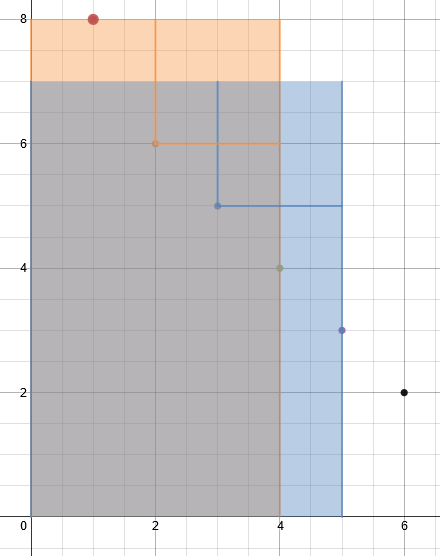
\includegraphics[width=.4\linewidth]{EjemploArea4}
  \caption{Área de impacto de B en naranja y de C en azul.}
  \label{fig:test1}
\end{minipage}%
\begin{minipage}{.5\textwidth}
  \centering
  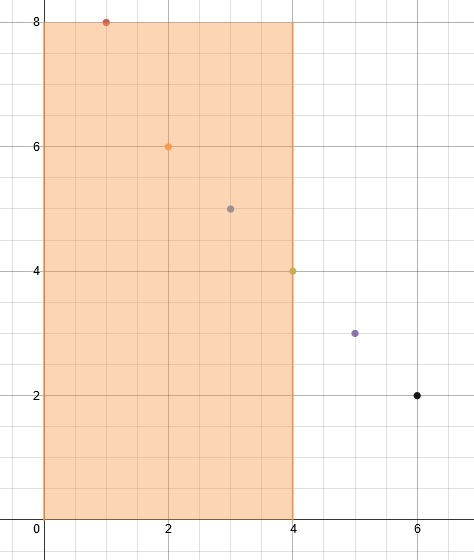
\includegraphics[width=4cm]{EjemploArea5}
  \caption{Área de impacto de B en naranja.}
  \label{fig:test2}
\end{minipage}

\begin{minipage}{.5\textwidth}
  \centering
  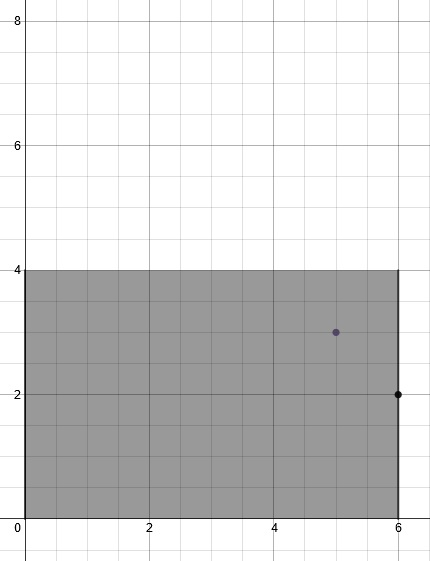
\includegraphics[width=4cm]{EjemploArea6}
  \caption{Área de impacto de F en negro.}
  \label{fig:test2}
\end{minipage}

\end{figure}

\newpage
\subsection{Ideas para desarrollar el algoritmo}

Definamos el área de impacto como
\begin{gather*}
\textrm{A}:\mathbb{N_{0}}^2 \times \mathbb{N} \rightarrow \mathbb{Z^2}\\
 \mathbf{A}(P,T) = \{ (x, y) \in \mathbb{Z^2} : 0 \leq x \leq P_{x}+T ~ \wedge ~ 0 \leq y \leq P_{y}+T \}
\end{gather*}
 es decir, el conjunto de puntos del plano en los que en caso de haber androides estos morirían por la Gendikama tirada en P. Con esta idea de área de impacto se puede pensar que no aporta tener en cuenta el área por sobre el objetivo vivo de mayor coordenada en y.
Va a haber que eliminar al objetivo situado en A. Se puede tirar una Gendikama al punto A, pero surge la pregunta de si se podría hacer algo mejor. ¿Qué pasa si se dispara a B? Si $ A_{y} \leq B_{y}+T$ entonces el área de impacto A(B,T) incluye al punto A. Así, sería mejor disparar la Gendikama a B que a A dado que como  $A_{x} < B_{x}$ entonces  $A_{x}+T < B_{x}+T$, lo que nos da una idea intuitiva de inclusión de áreas, $A(A,T) \subset A(B,T)$ (nótese que la inclusión es estricta) y podemos decir que diparar a B es más destructivo.
Así, volvemos a preguntarnos: ¿Qué pasa si se dispara a C? ¿Esto también mataría a A?
Si sí, seguimos preguntándonos por el siguiente punto de menor coordenada y, y podemos tener dos situaciones:

\begin{itemize}
\item[•] Recorrer hasta el último punto y que una Gendikama lanzada ahí también elimine al androide situado en A, necesitando sólo un disparo para destruir a todos.
\item[•] Recorrer hasta eventualmente encontrar un androide posicionado en un punto $K$ al que si se lanzara una Gendikama ésta no matara al androide en A. En este caso habría que disparar al androide situado en la posición con la coordenada $y$ inmediatamente anterior a la de $K$, llamémoslo J, y calcular $J_{x}+T$ para ver cuál sería el objetivo de mayor coordenada $y$ que quedara vivo  y repetir el proceso como si este fuera el nuevo $A$. Si no quedara ningún objetivo por eliminar entonces ya no habría necesidad de seguir disparando Gendikamas.
\end{itemize}

\subsection{Pseudocódigo}
\begin{algorithm}
\caption{IndiceDeMenorYQueLoMata}
\begin{algorithmic}
  \Function{IndiceDeMenorYQueLoMata}{t: int, indiceDeObjetivo: int, e: $Arreglo<Tupla<int,int>>$} $\to j$ : \texttt{int}
	\State $int~ j \gets indiceDeObjetivo - 1$ \Comment $\mathcal{O}(1)$
	\While{$(j \geq 0) \wedge (((e[j]).y + t) \geq (e[indiceDeObjetivo]).y)$} \Comment $\mathcal{O}(indiceDeObjetivo)$
		\State j-~- \Comment $\mathcal{O}(1)$
	\EndWhile
	\State j++ \Comment $\mathcal{O}(1)$
	\State return j \Comment $\mathcal{O}(1)$
\EndFunction
\end{algorithmic}
\underline{Complejidad:} $\mathcal{O}(indiceDeObjetivo)$\\
    
\end{algorithm}

\begin{algorithm}
\caption{IndiceDeMayorXQueMata}
\begin{algorithmic}
  \Function{IndiceDeMayorXQueMata}{t: int, indiceDeObjetivo: int, e: $Arreglo<Tupla<int,int>>$} $\to j$ : \texttt{int}
  	\State $int~ distanciaDeDano \gets e[indiceDeObjetivo].x + t$ \Comment $\mathcal{O}(1)$
	\State $int~ i \gets indiceDeObjetivo - 1$ \Comment $\mathcal{O}(1)$
	\While{$(i \geq 0) \wedge (((e[i]).x) \leq distanciaDeDano$} \Comment $\mathcal{O}(indiceDeObjetivo)$
		\State i-~- \Comment $\mathcal{O}(1)$
	\EndWhile
	\State i++ \Comment $\mathcal{O}(1)$
	\State return i \Comment $\mathcal{O}(1)$
\EndFunction
\end{algorithmic}
\underline{Complejidad:} $\mathcal{O}(indiceDeObjetivo)$\\
    
\end{algorithm}
\newpage

\begin{algorithm}
\caption{Genkidama}
\begin{algorithmic}
  \Function{Genkidama}{t: int, n: int, e: $Arreglo<Tupla<int,int>>$}
  	\State $int~[~]~ atacados$ \Comment $\mathcal{O}(1)$
  	\State $int ~genkidamasUtilizadas \gets 0$ \Comment $\mathcal{O}(1)$
	\State $int ~indiceDeObjetivoPorArea \gets n - 1$ \Comment $\mathcal{O}(1)$
	\State $ //~el~ de~ arriba~ es~ aquel~ al~ que~ quiero~ que~ le~ llegue~ la~ onda~ expansiva$
	\State $bool ~hayAlgunoVivo \gets true$ \Comment $\mathcal{O}(1)$
	\While{$hayAlgunoVivo$} \Comment $\mathcal{O}(indiceDeObjetivo)$
		\State $ 	//~el~ de~ abajo ~es~ aquel~ al~ que~ le~ voy~ a ~tirar~ la~ bomba$
		\State $int~indiceDeMenorYQueLoMata(t, indiceDeObjetivoPorArea, e)$ \Comment $\mathcal{O}(indiceDeObjetivoPorArea)$
		\State $agregarAtras(atacados, indiceDeObjetivo + 1)$ \Comment $\mathcal{O}(1)$
		\State $		//~el +1 ~de~ arriba~ surge~ de~ que~ en~ el~ enunciado ~se~ enumeran~ desde~ el~ 1 ~$
		\State $	   y~ nosotros~ enumeramos~ desde~ 0$
		\State $hayAlgunoVivo \gets \neg(indiceDeMayorXQueMata(t, indiceDeObjetivo, e) == 0)$ \Comment $\mathcal{O}(indiceDeObjetivo)$
		\State $indiceDeObjetivoPorArea \gets indiceDeMayorXQueMata(t, indiceDeObjetivo, e) - 1$ \Comment $\mathcal{O}(indiceDeObjetivo)$
		\State genkidamasUtilizadas++ \Comment $\mathcal{O}(1)$
	\EndWhile
	\State $imprimir ~genkidamasUtilizadas$
	\State $int~ h \gets 0$
	\While{$h < genkidamasUtilizadas$}
			\State $imprimir ~atacados[h]$
			\State $h++$
			\If{$h < genkidamasUtilizadas$}
					\State $imprimir ~"~"~$
			\EndIf
	\EndWhile
\EndFunction
\end{algorithmic}
\underline{Complejidad:} $\mathcal{O}(indiceDeObjetivo)$\\
    
\end{algorithm}

\newpage

\subsection{Cota de complejidad}
Como se puede ver en el pseudocódigo y se explica en la sección "Ideas para desarrollar el algoritmo" se recorren todos los puntos ordenados, de mayor a menor coordenada $y$, una vez, ya sea para encontrar a que enemigo atacar o para ver cuales murieron en el último ataque.
Cuando se busca un enemigo a atacar, se verifica que al atacarlo se maten todos los anteriores, así al lanzar una Genkidama sabemos que todos los enemigos por los que ya iteramos estarán muertos y solo queda ver cuales de los siguentes al enemigo atacado tambíen muerieron. Esto se logra iterando por los enemigos subsiguientes al atacado hasta encontrar el primero al que la Genkidama no mató y con él se vuelve a comenzar el proceso. Se puede ver claramente que se itera por todos los enemigos y que se hace solo una vez haciendo que la complejidad sea $\mathcal{O}(n)$ siendo $n$ la cantidad de enemigos.

\subsection{Experimentacion}
\begin{verbatim}
Acontinuacion se informa detalladamente el experimento que se hizo. Para hacer mas facil la lectura, hay que notar la cantidad de puntos fue aumentando, para sada cantidad se realizaron 2 mediciones, porque la resolucion del problema esta muy relacionada con los puntos que se generan. Se ve que los tiempos aumentan cuanto mas grande es la cantidad de puntos y para instancias grandes varia bastante. Luego del experimento se presenta un grafico.

cantidad de puntos = 10
t = 1
posiciones de los puntos = 95  11 - 86  24 - 81  40 - 58  50 - 56  51 - 52  54 - 43  57 - 28  62 - 21  76 - 19  90
el tiempo fue 3.3e-05
genkidamasUtilizadas  = 9
atacados : 10 9  8  7  6  4  3  2  1

cantidad de puntos = 10
t = 1
posiciones de los puntos = 98  10 - 97  30 - 88  39 - 87  40 - 83  60 - 80  64 - 77  66 - 24  76 - 13  86 - 3  87
el tiempo fue 3e-05
genkidamasUtilizadas 7
atacados 9  8  7  6  5  3  2

cantidad de puntos = 20
t = 3
posiciones de los puntos = 99  1 - 81  3 - 80  14 - 77  15 - 63  21 - 62  24 - 61  26 - 47  30 - 44  39 - 37  50 - 30  59 - 28  66 - 26  73 - 25  78 - 23  79 - 22  88 - 14  89 - 13  93 - 10  94 - 0  98
el tiempo fue 4.7e-05
genkidamasUtilizadas 10
atacados 20  18  16  13  11  10  9  6  3  1

cantidad de puntos = 20
t = 3
posiciones de los puntos = 94  0 - 92  20 - 91  25 - 90  26 - 86  31 - 84  36 - 75  40 - 73  42 - 58  54 - 51  57 - 30  63 - 26  64 - 24  67 - 22  68 - 20  70 - 17  72 - 16  73 - 4  79 - 1  91 - 0  94
el tiempo fue 2.5e-05
genkidamasUtilizadas 8
atacados 19  15  12  11  9  7  6  3

cantidad de puntos = 30
t = 2
posiciones de los puntos = 96  2 - 93  4 - 90  5 - 89  6 - 88  9 - 86  11 - 84  14 - 81  15 - 80  19 - 70  20 - 68  21 - 64  29 - 60  33 - 56  37 - 49  38 - 47  40 - 42  42 - 39  50 - 35  60 - 28  62 - 24  66 - 22  67 - 21  69 - 16  73 - 15  76 - 14  83 - 10  85 - 8  93 - 4  96 - 3  99
el tiempo fue 0.000141
genkidamasUtilizadas 14
atacados 30  28  26  22  19  18  16  14  13  12  9  7  5  1

cantidad de puntos = 30
t = 2
posiciones de los puntos = 89  1 - 87  7 - 84  13 - 82  22 - 80  23 - 75  24 - 70  25 - 64  34 - 61  39 - 58  46 - 55  49 - 54  50 - 52  55 - 49  57 - 48  59 - 43  60 - 41  61 - 39  65 - 38  66 - 35  71 - 33  85 - 27  86 - 24  90 - 21  92 - 14  93 - 11  94 - 10  95 - 4  97 - 3  98 - 0  99
el tiempo fue 8.4e-05
genkidamasUtilizadas 14
atacados 28  25  23  21  18  15  13  11  10  9  8  5  3  2

Grafico
%%aca se agrega el grafico
\end{verbatim}

\newpage
\subsection{Apéndice: código de Genkidama}
\begin{lstlisting}
#include <tuple>
#include <vector>
#include <iostream>
#include <cassert>
using namespace std;

void genkidama(int, int, vector<tuple<int, int>>);
int indiceDeMenorYQueLoMata(int, int, vector<tuple<int,int>>);
int indiceDeMayorXQueMata(int, int, vector<tuple<int,int>>);

int main(){
	int t;
	int n;
	cin >> n >> t;
	vector<tuple<int,int>> e;
	tuple<int,int> en;
	int x;
	int y;
	for (int i = 0; i < n; i++) {
		cin >> x >> y;
		en = make_tuple(x,y);
		e.push_back((en));
	}
	genkidama(t, n, e);
	return 0;
}

// Toma el t, el indice del objetivo en e y el vector de tuplas.
int indiceDeMenorYQueLoMata(int t, int indiceDeObjetivo, vector<tuple<int,int>> e){
	int j = indiceDeObjetivo - 1;
	while((j >= 0) && ((get<1>(e[j]) + t) >= get<1>(e[indiceDeObjetivo]))){
		j--;
	}
	j++;
	return j;
}

int indiceDeMayorXQueMata(int t, int indiceDeObjetivo, vector<tuple<int,int>> e){
	int distanciaDeDano = get<0>(e[indiceDeObjetivo]) + t;
	int i = indiceDeObjetivo - 1;
	while((i >= 0) && (get<0>(e[i]) <= distanciaDeDano)){
		i--;
	}
	i++;
	return i;
}

void genkidama(int t, int n, vector<tuple<int,int>> e){
	assert (n > 0 && n == e.size() && "La cantidad de enemigos es distinta a la cantidad de posisciones");
	vector<int> atacados;
	int genkidamasUtilizadas = 0;
	int indiceDeObjetivoPorArea = n-1;
	// el de arriba es aquel al que quiero que le llegue la onda expansiva
	bool hayAlgunoVivo = true;
	while(hayAlgunoVivo){
		// el de abajo es aquel al que le voy a tirar la bomba
		int indiceDeObjetivo = indiceDeMenorYQueLoMata(t, indiceDeObjetivoPorArea, e);
		atacados.push_back(indiceDeObjetivo + 1);
		// el +1 de arriba surge de que en el enunciado se enumeran desde el 1 y
		// nosotros enumeramos desde 0
		hayAlgunoVivo = !(indiceDeMayorXQueMata(t, indiceDeObjetivo, e) == 0);
		indiceDeObjetivoPorArea = indiceDeMayorXQueMata(t, indiceDeObjetivo, e) - 1;
		genkidamasUtilizadas++;
		
	}
	std::cout << genkidamasUtilizadas << std::endl;
	int h = 0;
	while (h < genkidamasUtilizadas) {
			std::cout << atacados[h];
			h++;
			if (h < genkidamasUtilizadas) {
					std::cout << " ";
			}
	}
	std::cout << std::endl;
}

\end{lstlisting}
\end{document}
